\section{Rethinking storage model for Docker registry}
\label{sec:file_adressable}

%\subsection{}
\paragraph{Benefit of file-level content addressable storage}
Docker registry can save a lot of space if using file-level content addressable storage. 
Benefit: saving money, reducing storage management overhead.

\subsection{File-level dedup model}

\begin{figure}
	\centering
	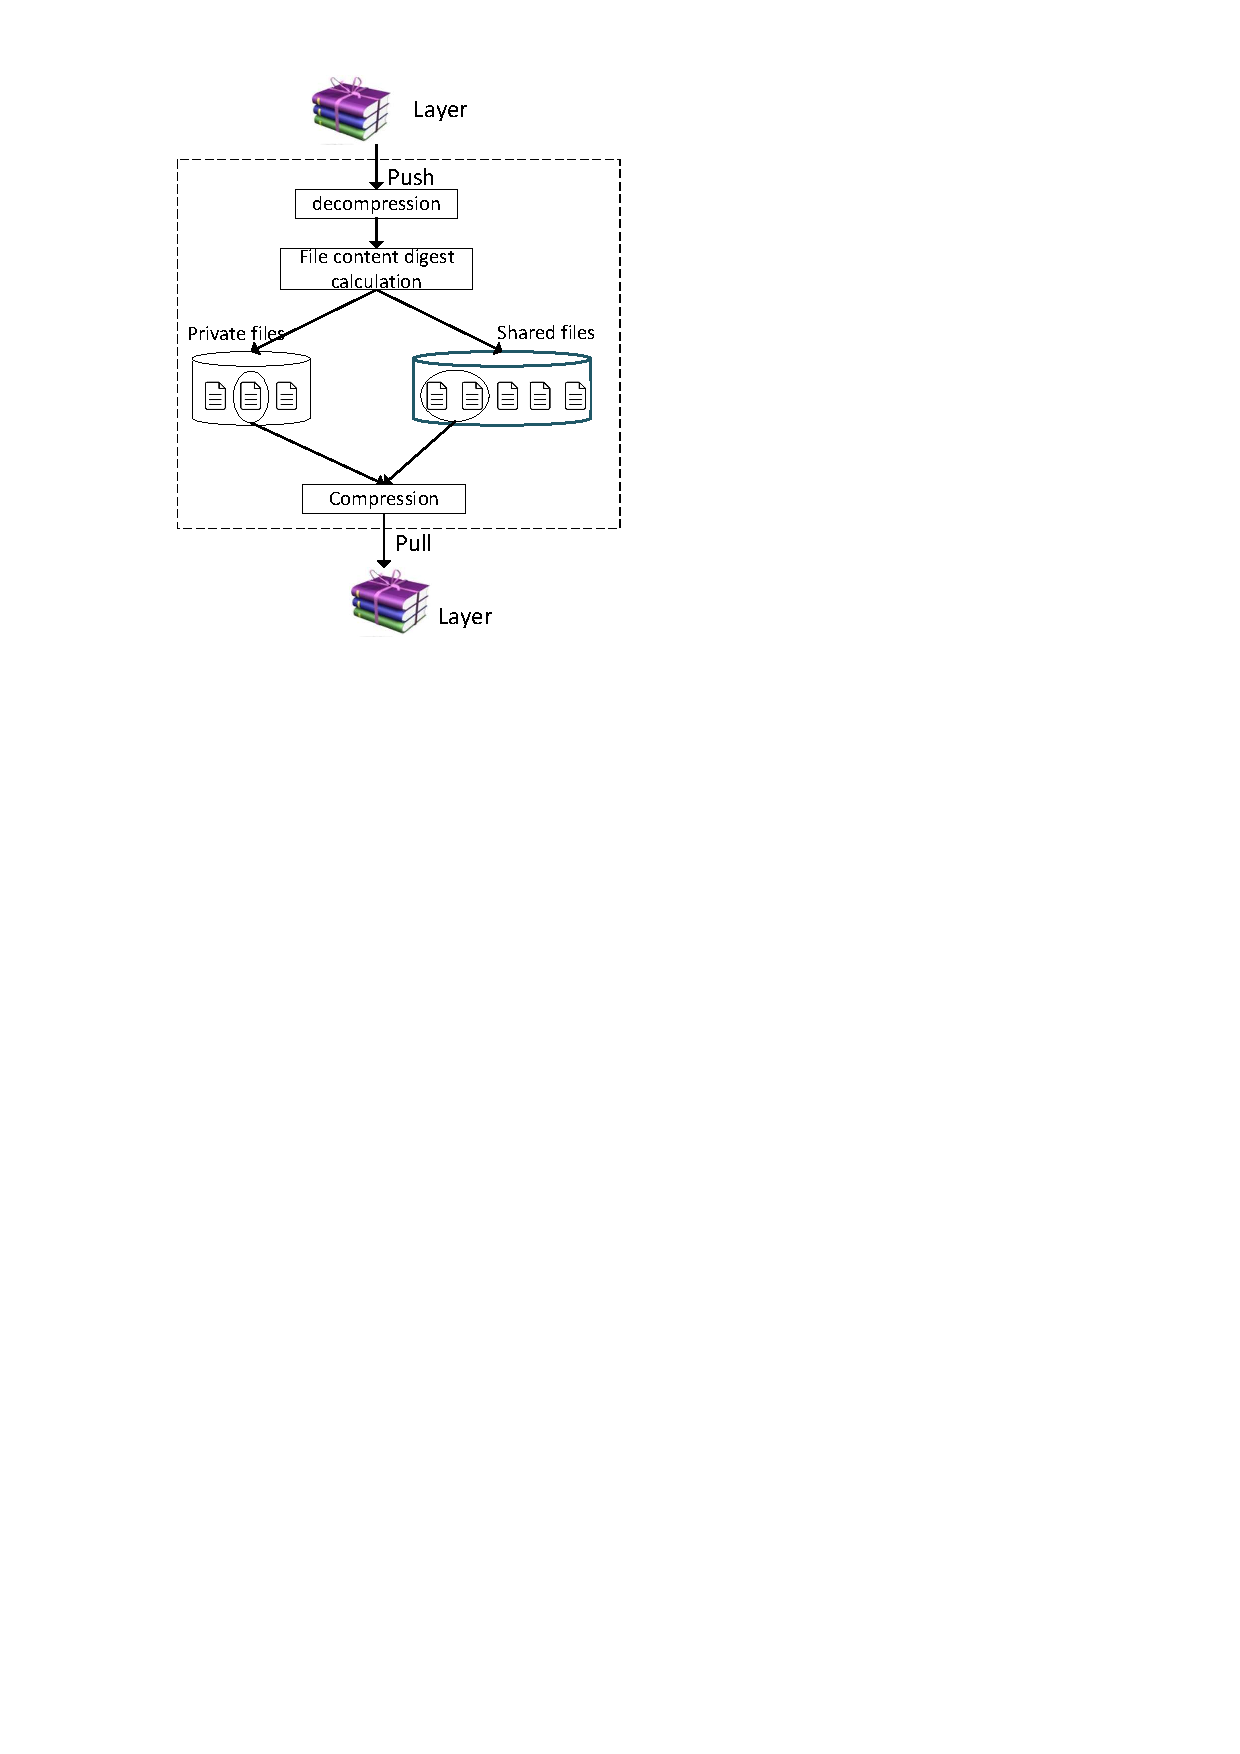
\includegraphics[width=0.3\textwidth]{graphs/graph_compression_layers.pdf}
	\caption{File-level dedup model.
	}
	\label{fig:file-dedup-model}
\end{figure}

\begin{figure}
	\centering
	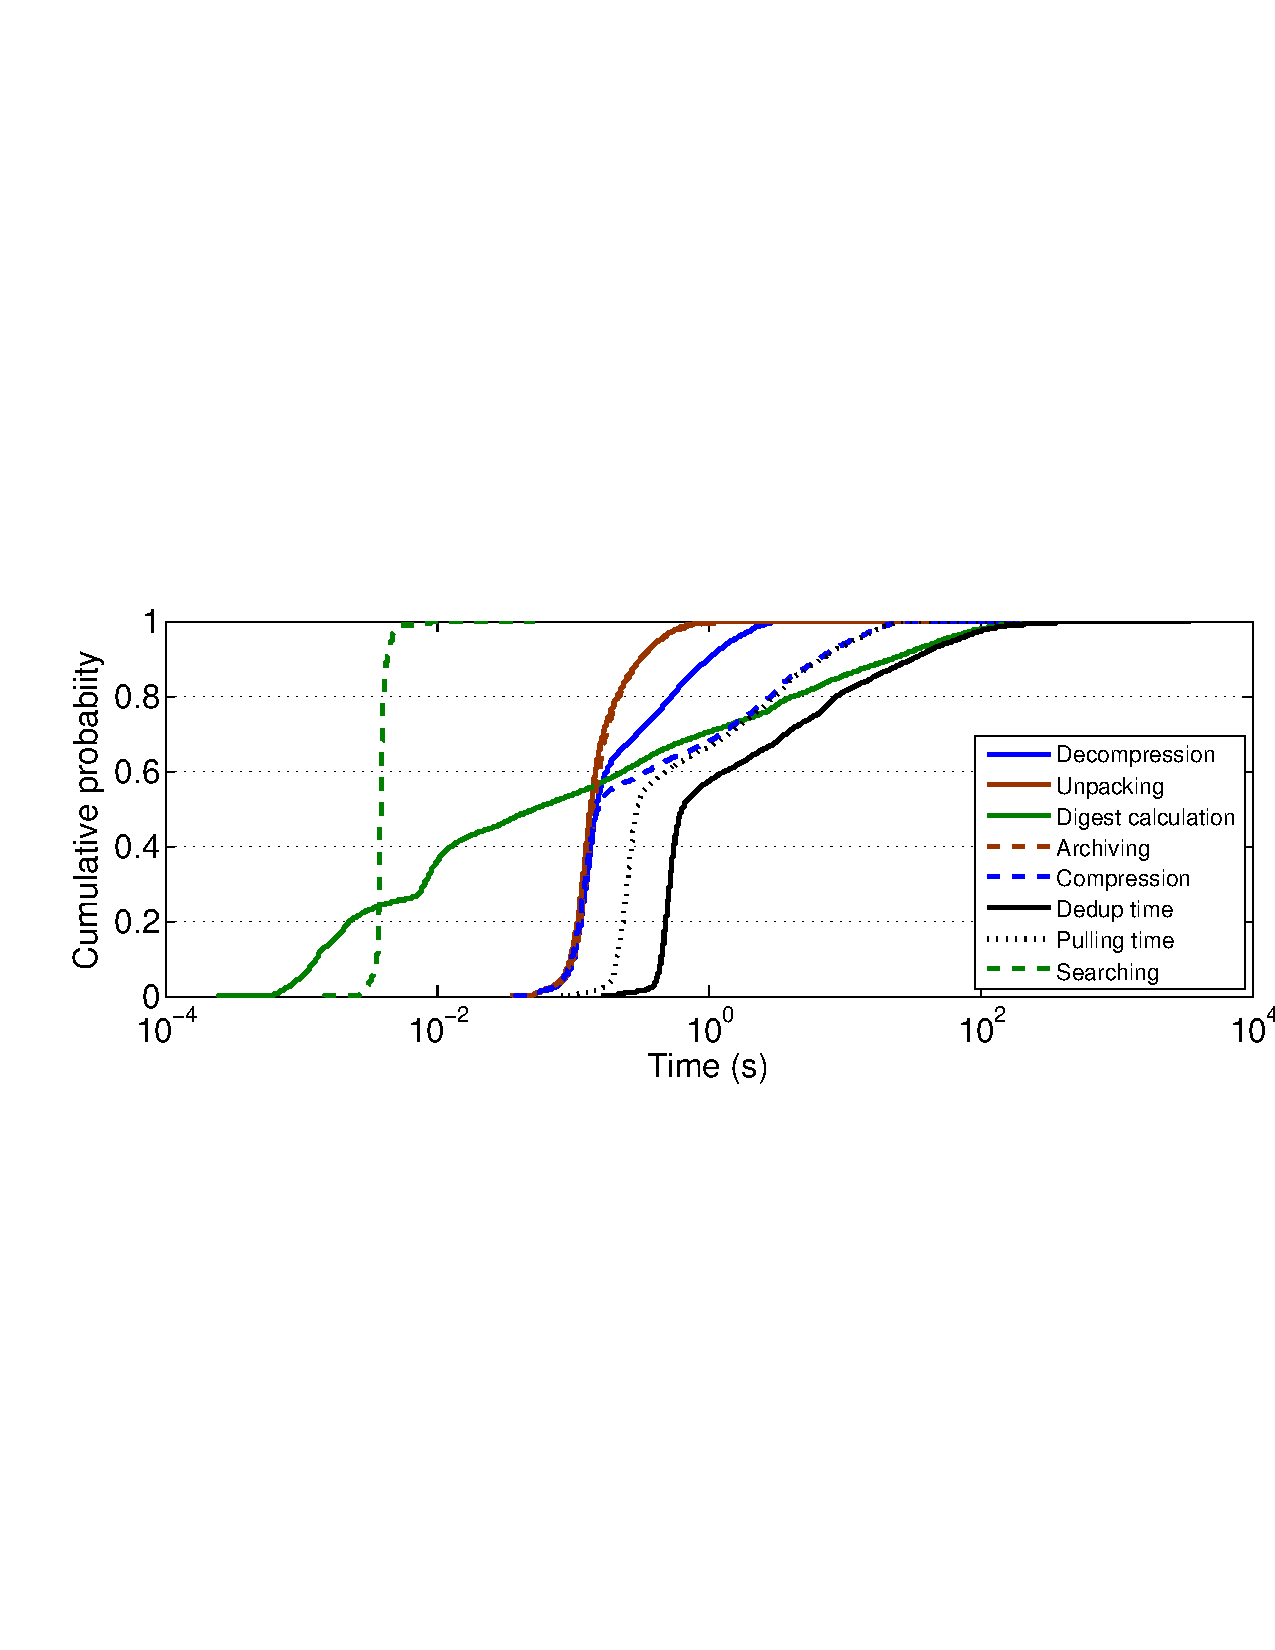
\includegraphics[width=0.3\textwidth]{graphs/res-time.pdf}
	\caption{File-level dedup model.
	}
	\label{fig:file-dedup-model}
\end{figure}

%\begin{figure}
%	\centering
%	\includegraphics [width=0.45\textwidth]{plots/exp-total-stev-erase.eps}
%	\subfigure[]{\label{fig:per_layer_ratio_fcnt_cdf}
%		\includegraphics [width=0.23\textwidth]{graphs/}
%	}
%	\subfigure[Similar layer dedup]{\label{fig:per_layer_ratio_fcnt_pdf}
%		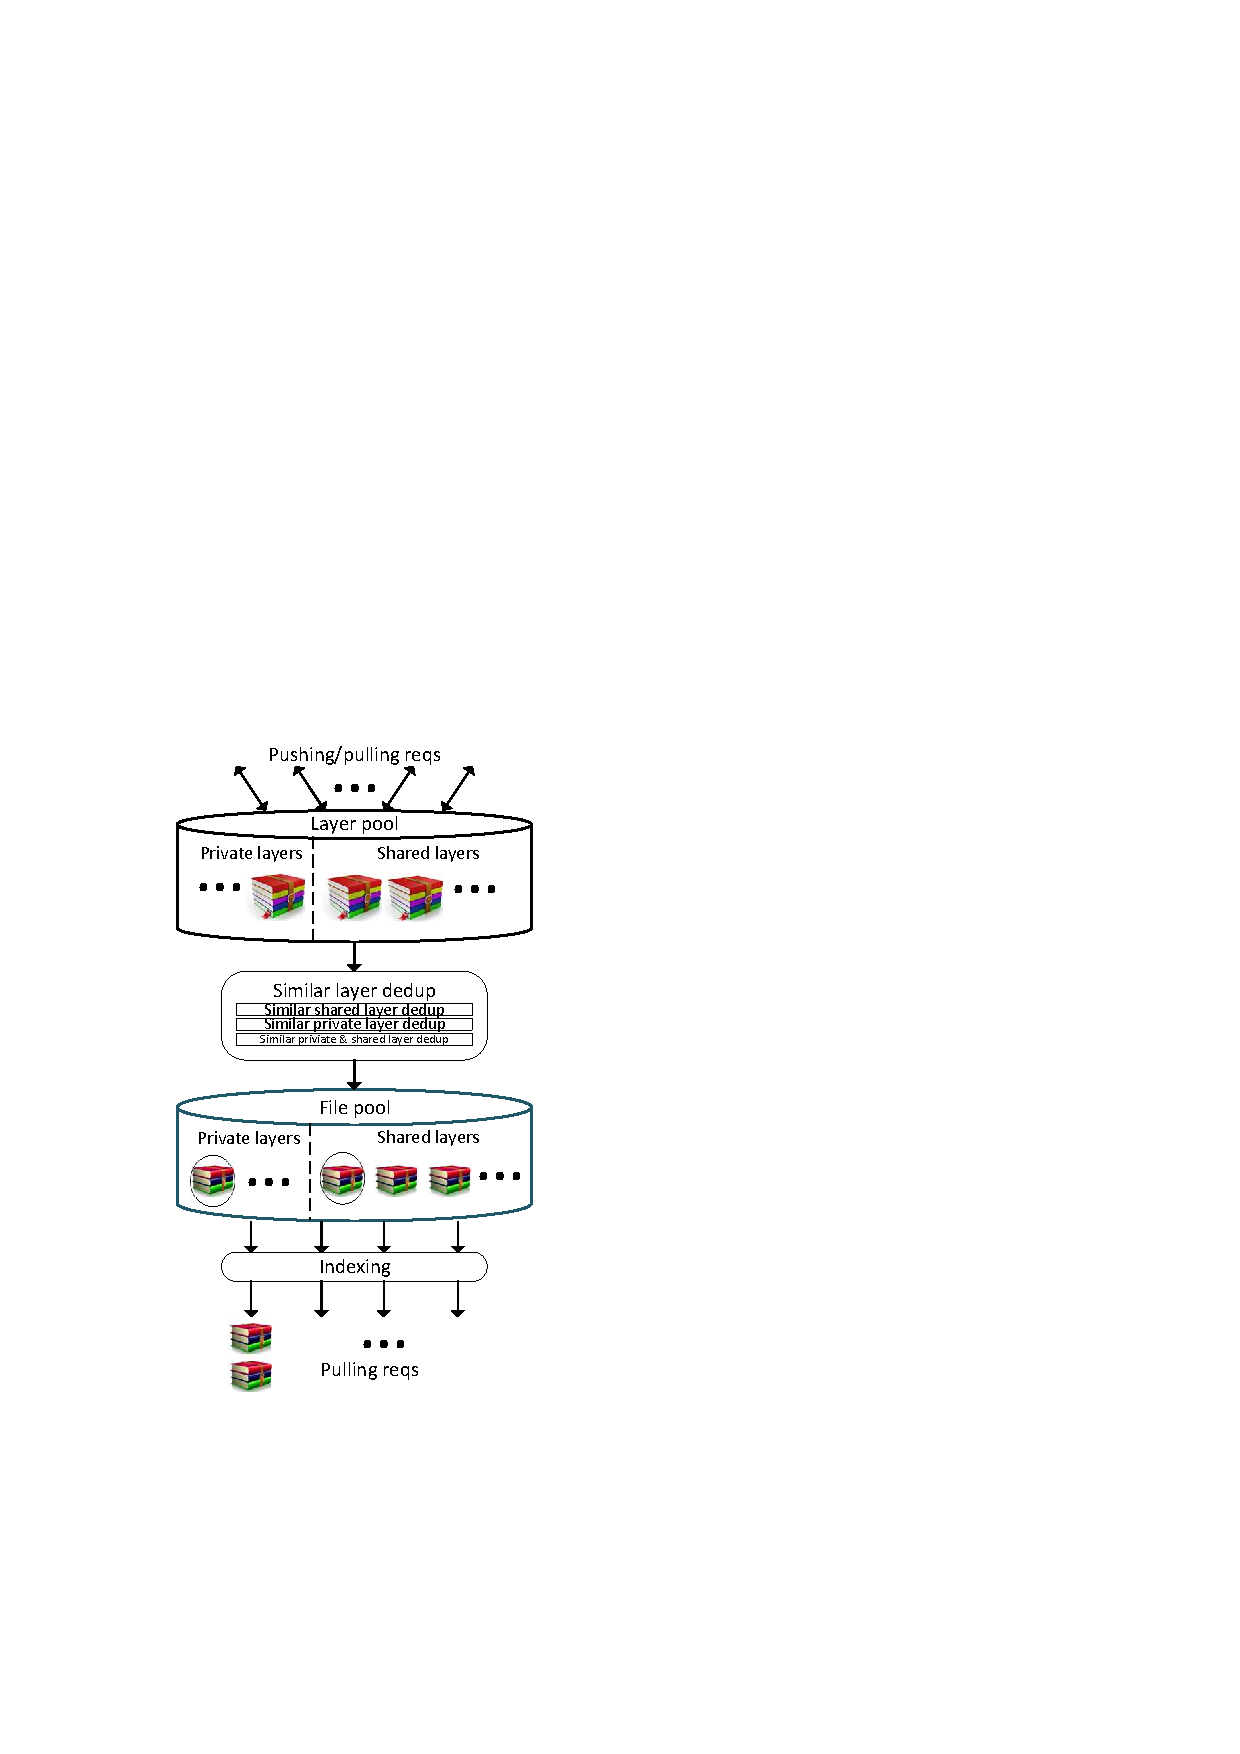
\includegraphics [width=0.22\textwidth]{graphs/graph_reconstruct_layers.pdf}
%	}
%	\caption{File-level content addressable storage model}
%	\label{fig:eval-stdev-erasure-cnt}
%\end{figure}

%\subsection{Hints for performance improvement and storage saving}

%\begin{table} 
%	\centering 
%	\scriptsize  
%	%\begin{minipage}{.5\linewidth}
%	\caption{Latency breakdown} \label{tbl:latency_breakdown} 
%	\begin{tabular}{|l|l|l|l|l|}%p{0.14\textwidth} 
%		\hline 
%		% after \\: \hline or \cline{col1-col2} \cline{col3-col4} ... 
%		% after \\: \hline or \cline{col1-col2} \cline{col3-col4} ... 
%		Operations/latency (S) & max & min & median & avg.\\
%		\hline
%		 gunzip decompression (RAM) & 257.16  & 0.04  & 0.15  & 0.39 \\
% 		\hline
% 		tar extraction (RAM) & 43.41  & 0.04  &  0.14  & 0.18 \\
%		\hline
%		Digest calculation (RAM) & 3455.01  & $<$0.00  & 0.05 & 10.65 \\
%		\hline
%		tar archiving (RAM)  & 53.44 & 0.04 & 0.14 & 0.19\\
%		\hline
%		gzip compression (RAM) & 496.04 & 0.04 & 0.15 & 2.10 \\
%%		\hline
%%		Total time (RAM) (with compression) & & & & \\
%%		\hline
%%		Total time (RAM) (without compression) & & & & \\
%		\hline
% 		\hline
% 		gunzip decompression (SSD) &   &   &    &  \\
% 		\hline
% 		tar extraction (SSD) &   &   &    &  \\
%		\hline
%		Digest calculation (SSD) &  &  & & \\
%		\hline
%		tar archiving (SSD) &  &  & & \\
%		\hline
%		gzip compression (SSD) & &  &  & \\
%%		\hline		 
%%		Total time (SSD) (with compression) & & & & \\
%%		\hline
%%		Total time (SSD) (without compression) & & & & \\
%		\hline
%		\hline
%		Network transfer & 20587.94 & $<$ 0.00 & $<$ 0.00 & 1.20 \\
%		\hline 	
%	\end{tabular} 
%\end{table}

\subsection{Trade-off discussion}

File-level dedup can reduce the redundant files in docker registry and save plenty of space. However, it also introduces considerable overhead, which including decompression, digest calculation, indexing, and compression overhead. These additional operations are either CPU intensive or I/O intensive. Thus, fast CPUs and high capacity RAM are required to improve performance.

We simulated a one-node docker registry with 64 RAM and 32 Cores. 
To improve performance, layers that are less than 50M are stored and processed in RAM while the rest layers are stored and processed in SSDs. Majority (87.3\%) of layers that are less than 50M are stored and processed in RAM.

Typically, workload fluctuates, with peaks and troughs. To reduce overhead, we can temporarily store the layers as gzip compressed tarball without file-level dedup when the workload is high while start file-level dedup when the workload is low. Consider that dedup is expensive in terms of performance overhead, file-level dedup is triggered when the workload is lower than $\sigma_{wl}$ and storage utilization is higher than $\sigma_{su}$.

\paragraph{Image \&. layer popularity skewness} 

%\begin{figure}[!t]
%	\centering
%	\subfigure[CDF of repositories by pull count]{\label{fig_pull_cnt_total}
%		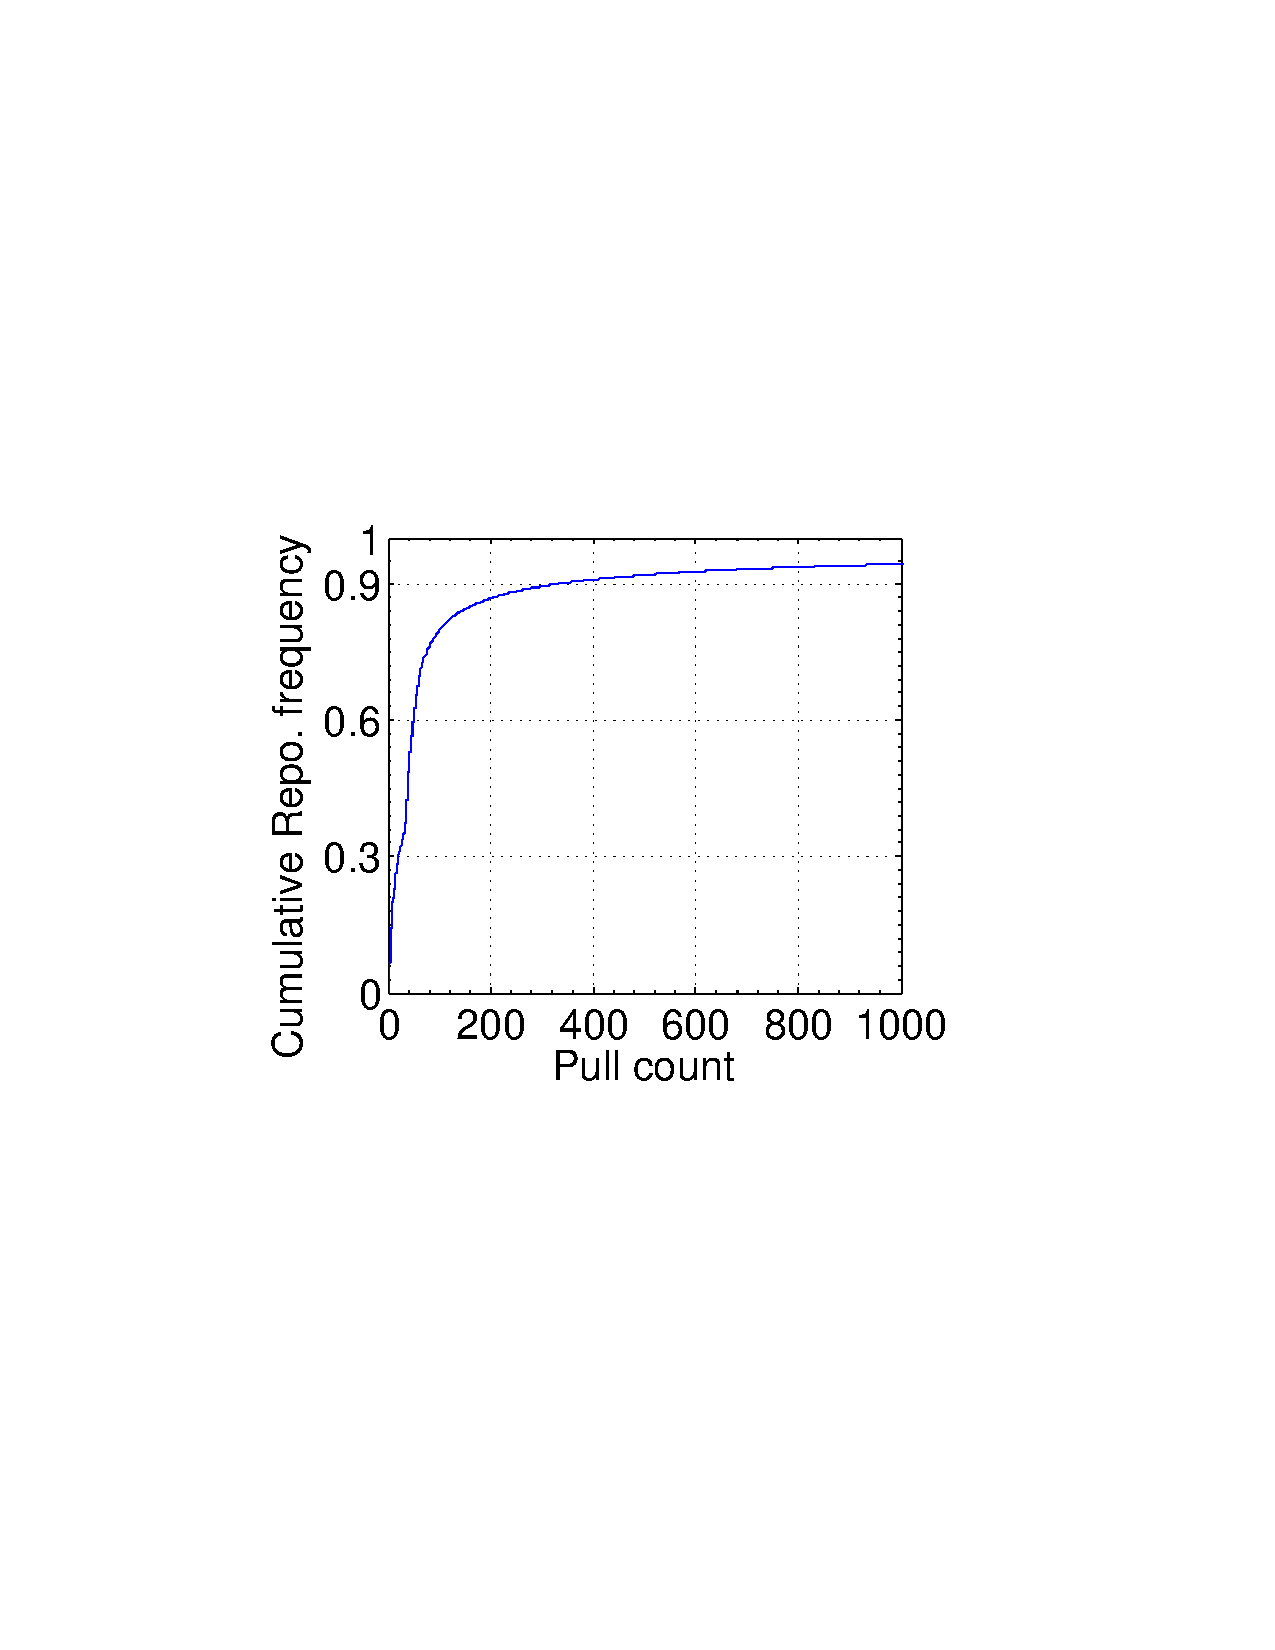
\includegraphics[width=0.23\textwidth]{graphs/pull_cnt.pdf}%
%	}
%	\subfigure[Histogram of repositories by pull count]{\label{fig_pull_cnt_count}
%		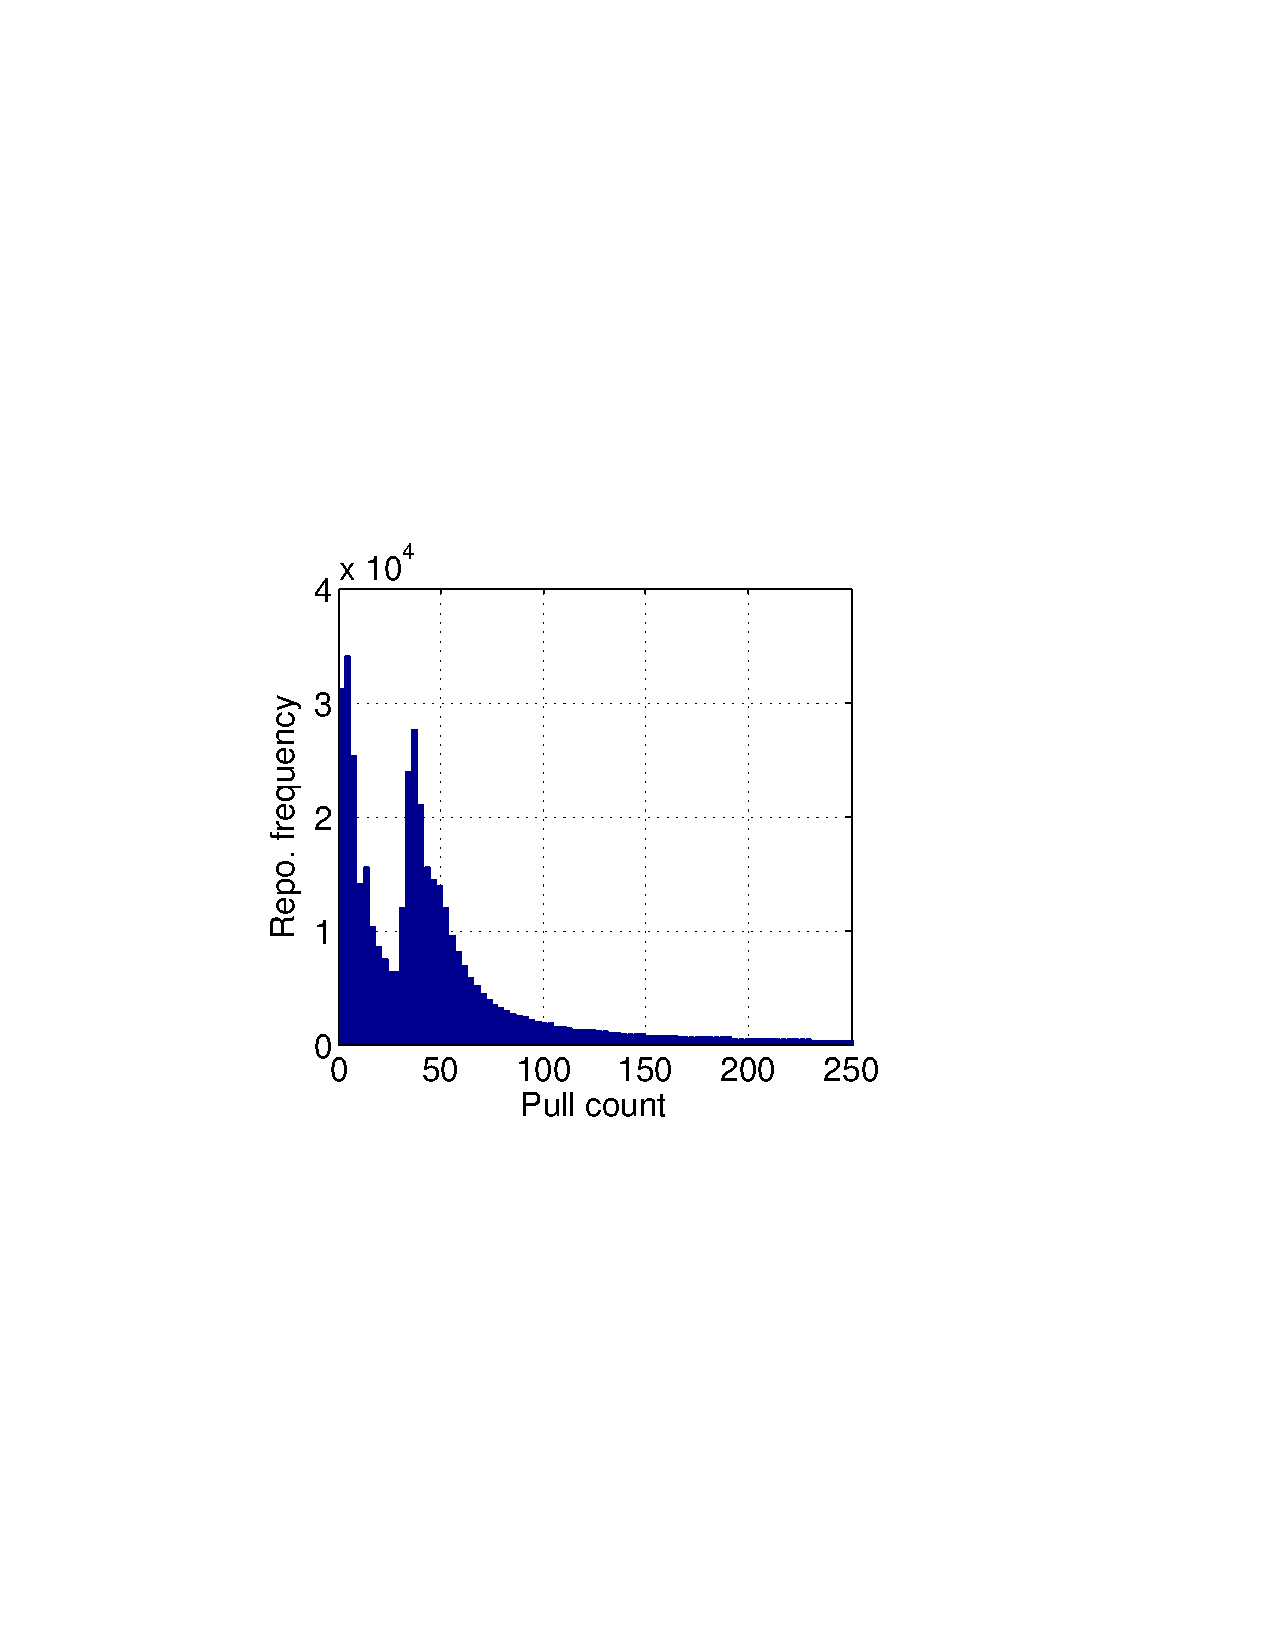
\includegraphics[width=0.22\textwidth]{graphs/count_pull_cnt.pdf}
%	}
%	\caption{Repository popularity distribution}
%	\label{fig-pop}
%\end{figure}

\begin{figure}
	\centering
	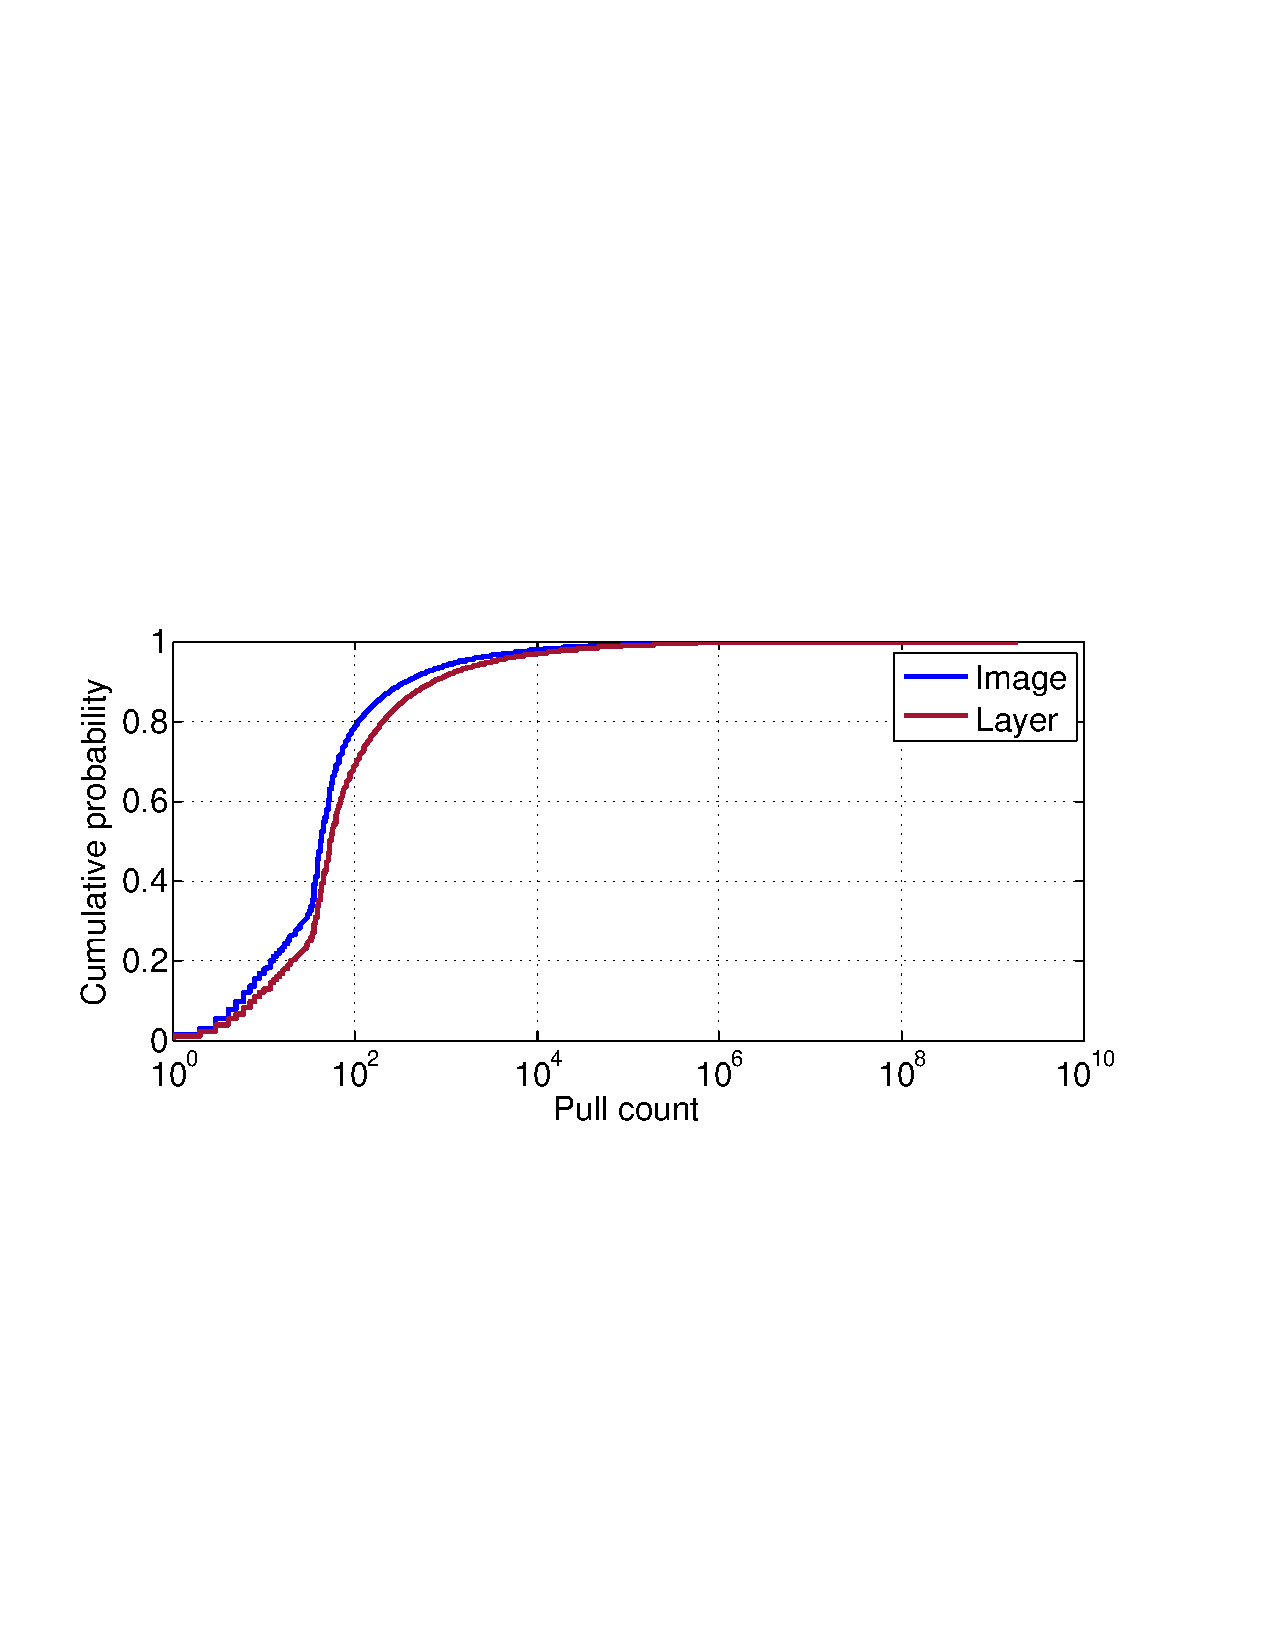
\includegraphics[width=0.4\textwidth]{graphs/pull-cnt.pdf}
	\caption{CDF of layer \& image pull count.
	}
	\label{fig:pull-cnt}
\end{figure}

x-axis shows the total number of pullings since the layers/images are stored in Docker Hub to May 30, 2017. Note that each layers'pull cnt. is calculated by aggregating all the images'pull cnts that refers this layer.

\subsubsection{Off-line file-level dedup latency} 
To quantify the overhead of file-level dedup, we measured its off-line performance by using file-level dedup for the whole dataset since dedup process only starts periodically when the workload is lower and only cold layers are evolved in dedup process (discussed in Section~\ref{xxx}). Figure~\cite{xxx} shows dedup latency and the breakdown latencies: decompression time, extraction time, and file digest calculation time.

First, majority (xxx) of layers'dedup times are less than xxx.
%during peak workload, which means that we start file-level dedup whenever it receives a layer. 
%To simulate the high intensive workload, we first sent a sequential of layer pushing requests to registry and stored, then we measure the file-level dedup  
To speed up dedup process, we leverage multi-processing. The throughput is 2.67 layers/s. 

Second, compare the latency for each operation, we see that xxxx
%\paragraph{Latency breakdown}

%We calculated the latency for each operation for all layers as shown as Table~\ref{tbl:latency_breakdown}.
 
\paragraph{Compression overhead for pulling}Note that the pushing performance wont be influenced by the file-level dedup because once the layer reaches registry, an response message will be sent to the user. No addition delay will be added to the pushing time. However, compression time will impact pulling performance since the files need to be compressed first and then sent to the users once registry receives pulling requests. 

Figure~\ref{xxx} shows the compression time across 
%\paragraph{Latency distribution for each operation}
%\subsubsection{When to start file-level dedup?} 

%\paragraph{Latency distribution for each operation}

%\paragraph{Small compression ratio and small layer size}
%
%\begin{figure}[!t]
	\centering
	\subfigure[CDF of compression ratio]{\label{fig_cdf_compression_ratio}
		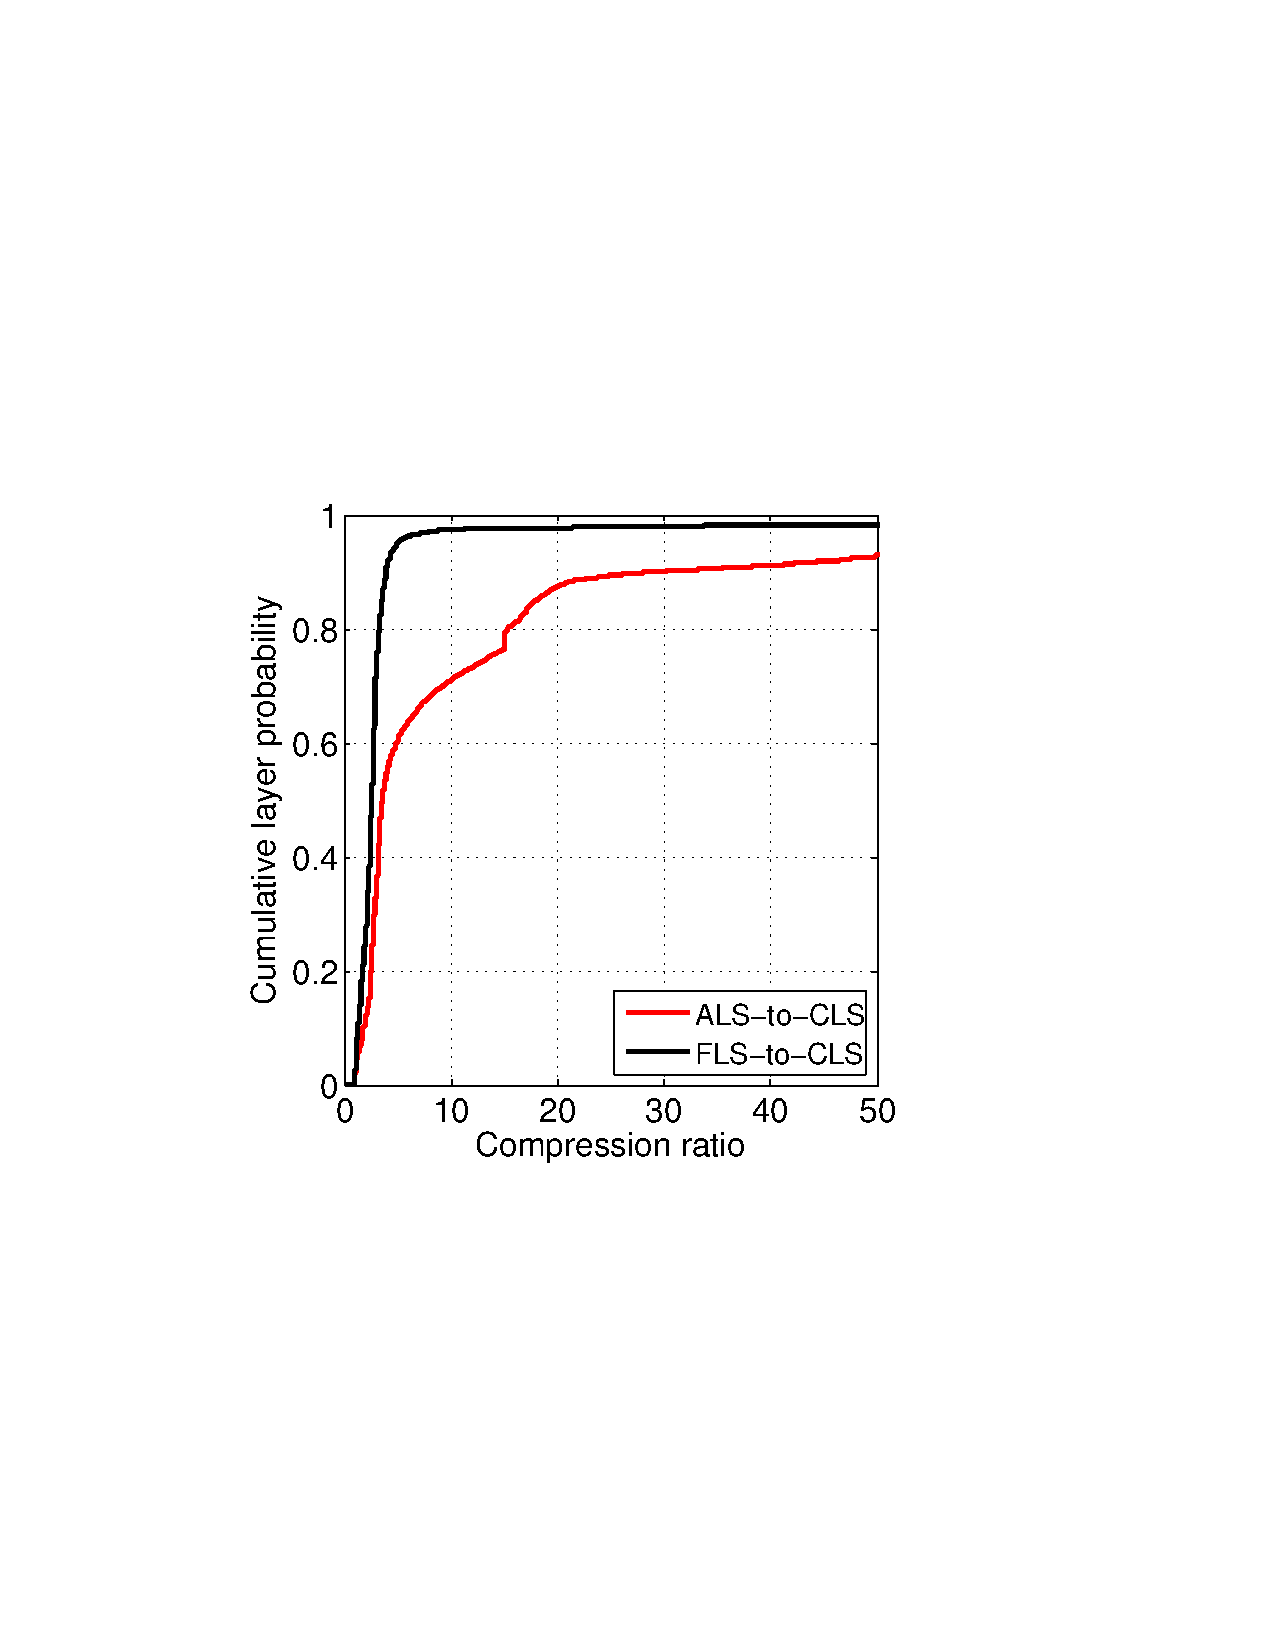
\includegraphics[width=0.23\textwidth]{graphs/cdf_compression_ratio.pdf}
	}
	\subfigure[Histogram of comp. ratios]{\label{fig_his_compression_ratio}
		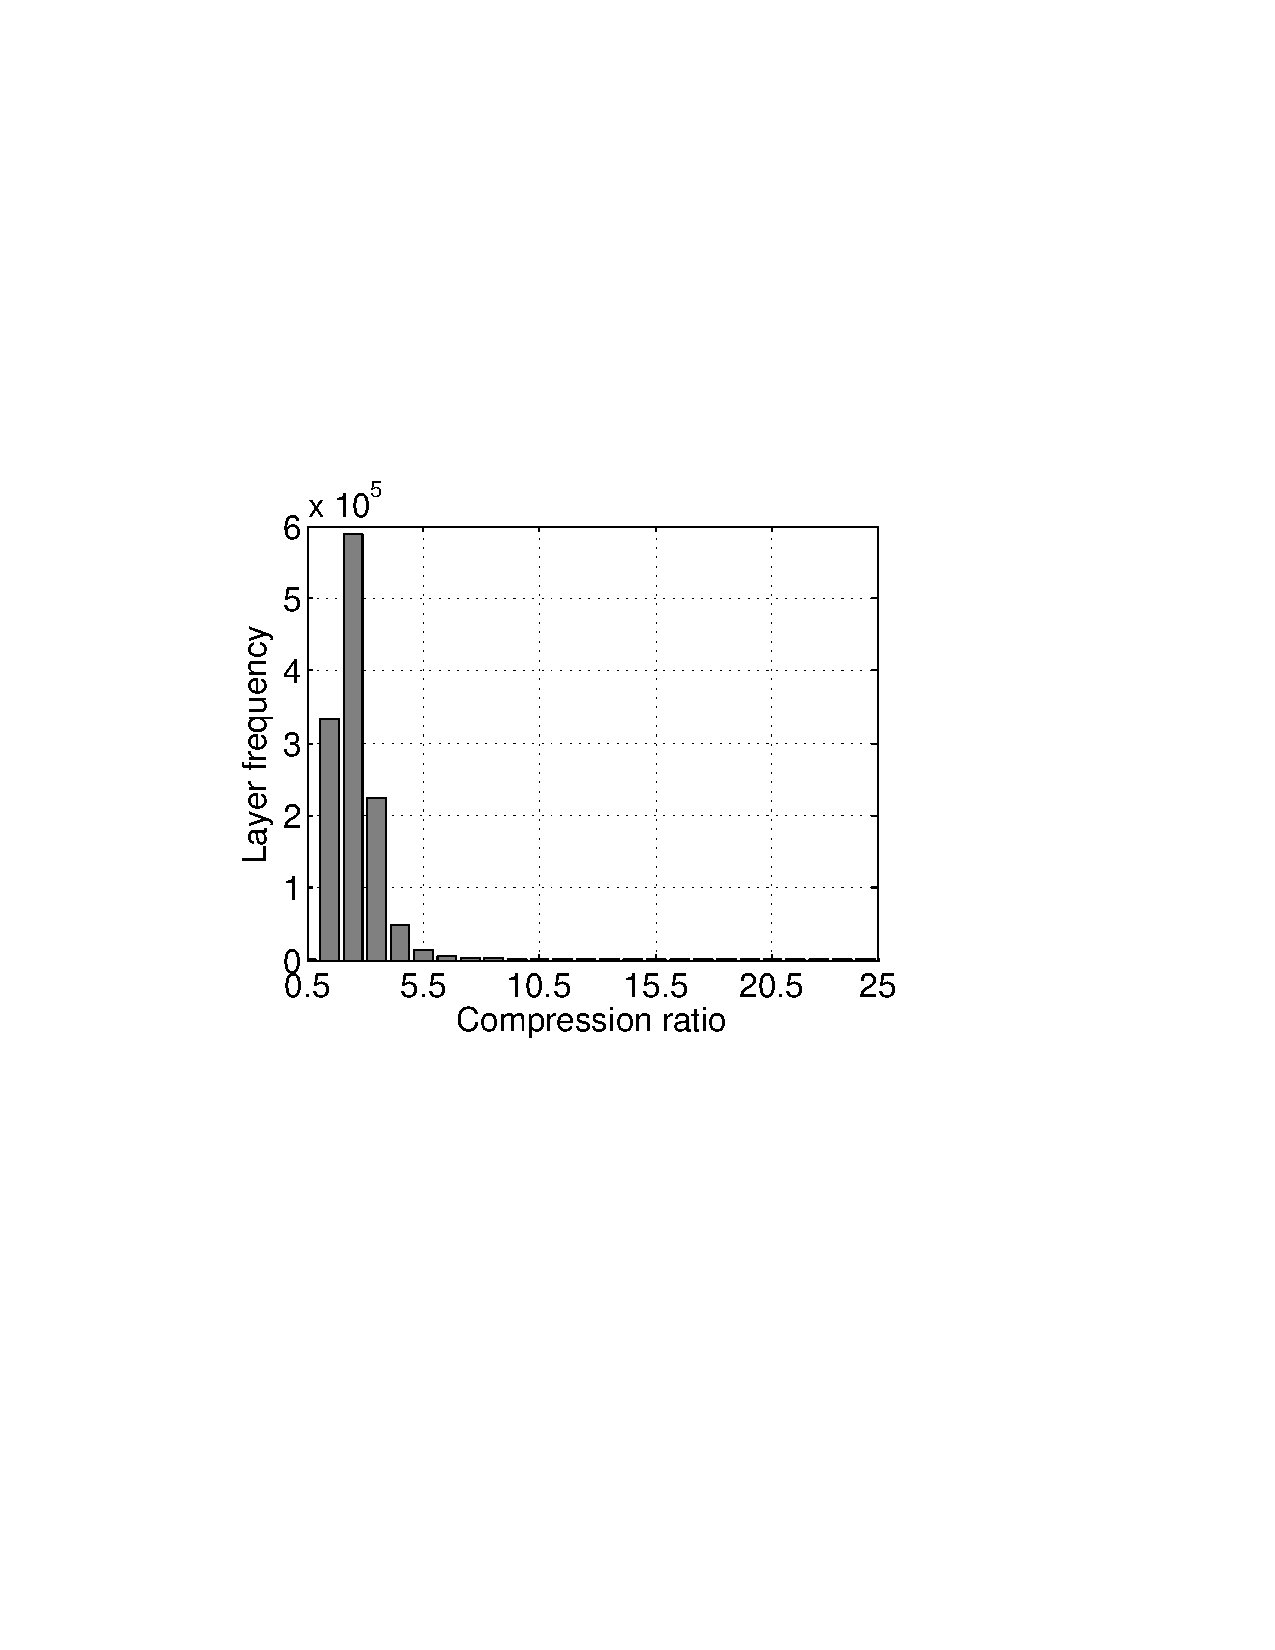
\includegraphics[width=0.223\textwidth]{graphs/his_compression_ratio.pdf}
	}
	\caption{Layer compression ratio distribution
	%\vcomment{Different colors are used in figure (a) and (b) FLS/CLS\nancomment{will address later}}
	}
	\label{fig-compression-ratio}
\end{figure}

%
%\begin{figure}[!t]
	\centering
	\subfigure[CDF of layer sizes]{\label{fig_layer_size_cdf}
		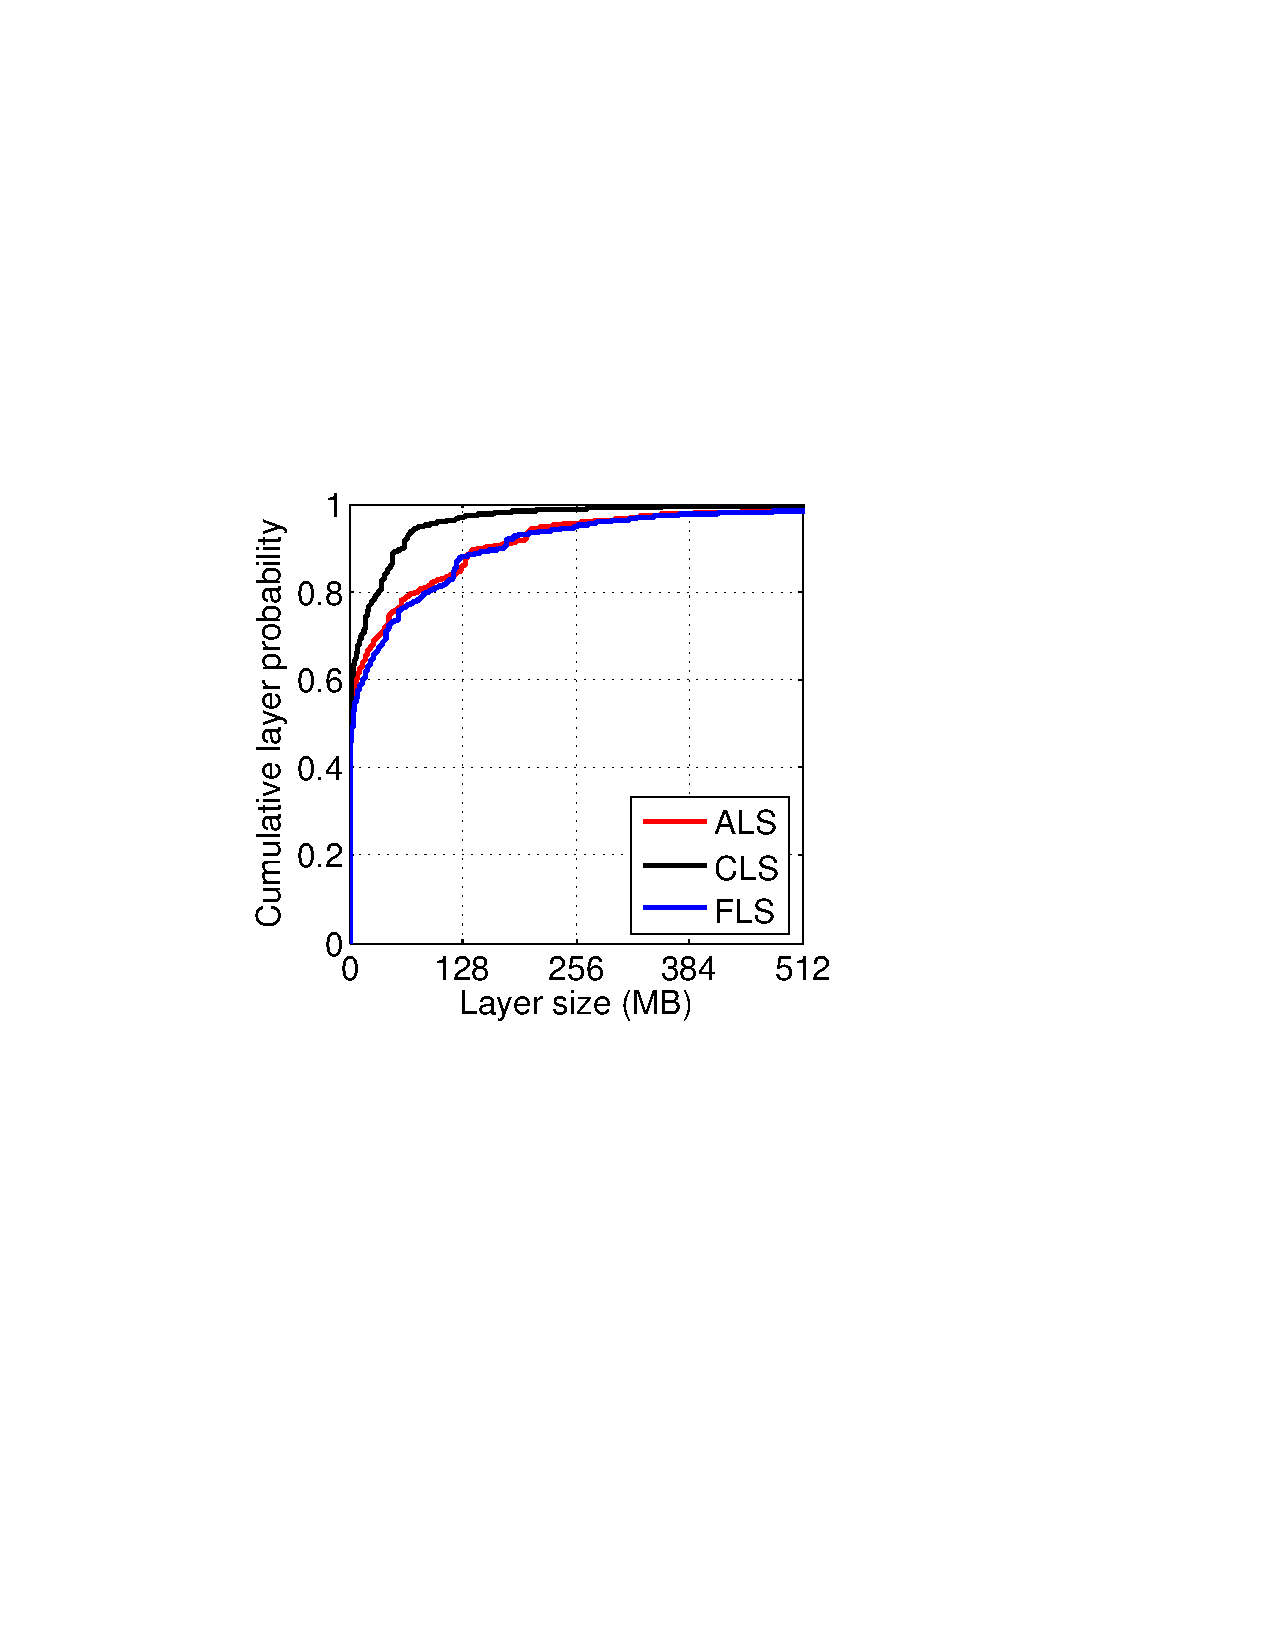
\includegraphics[width=0.234\textwidth]{graphs/layer_size_mb.pdf}
	}
	\subfigure[Histogram of layer sizes]{\label{fig_hist_layer_size}
		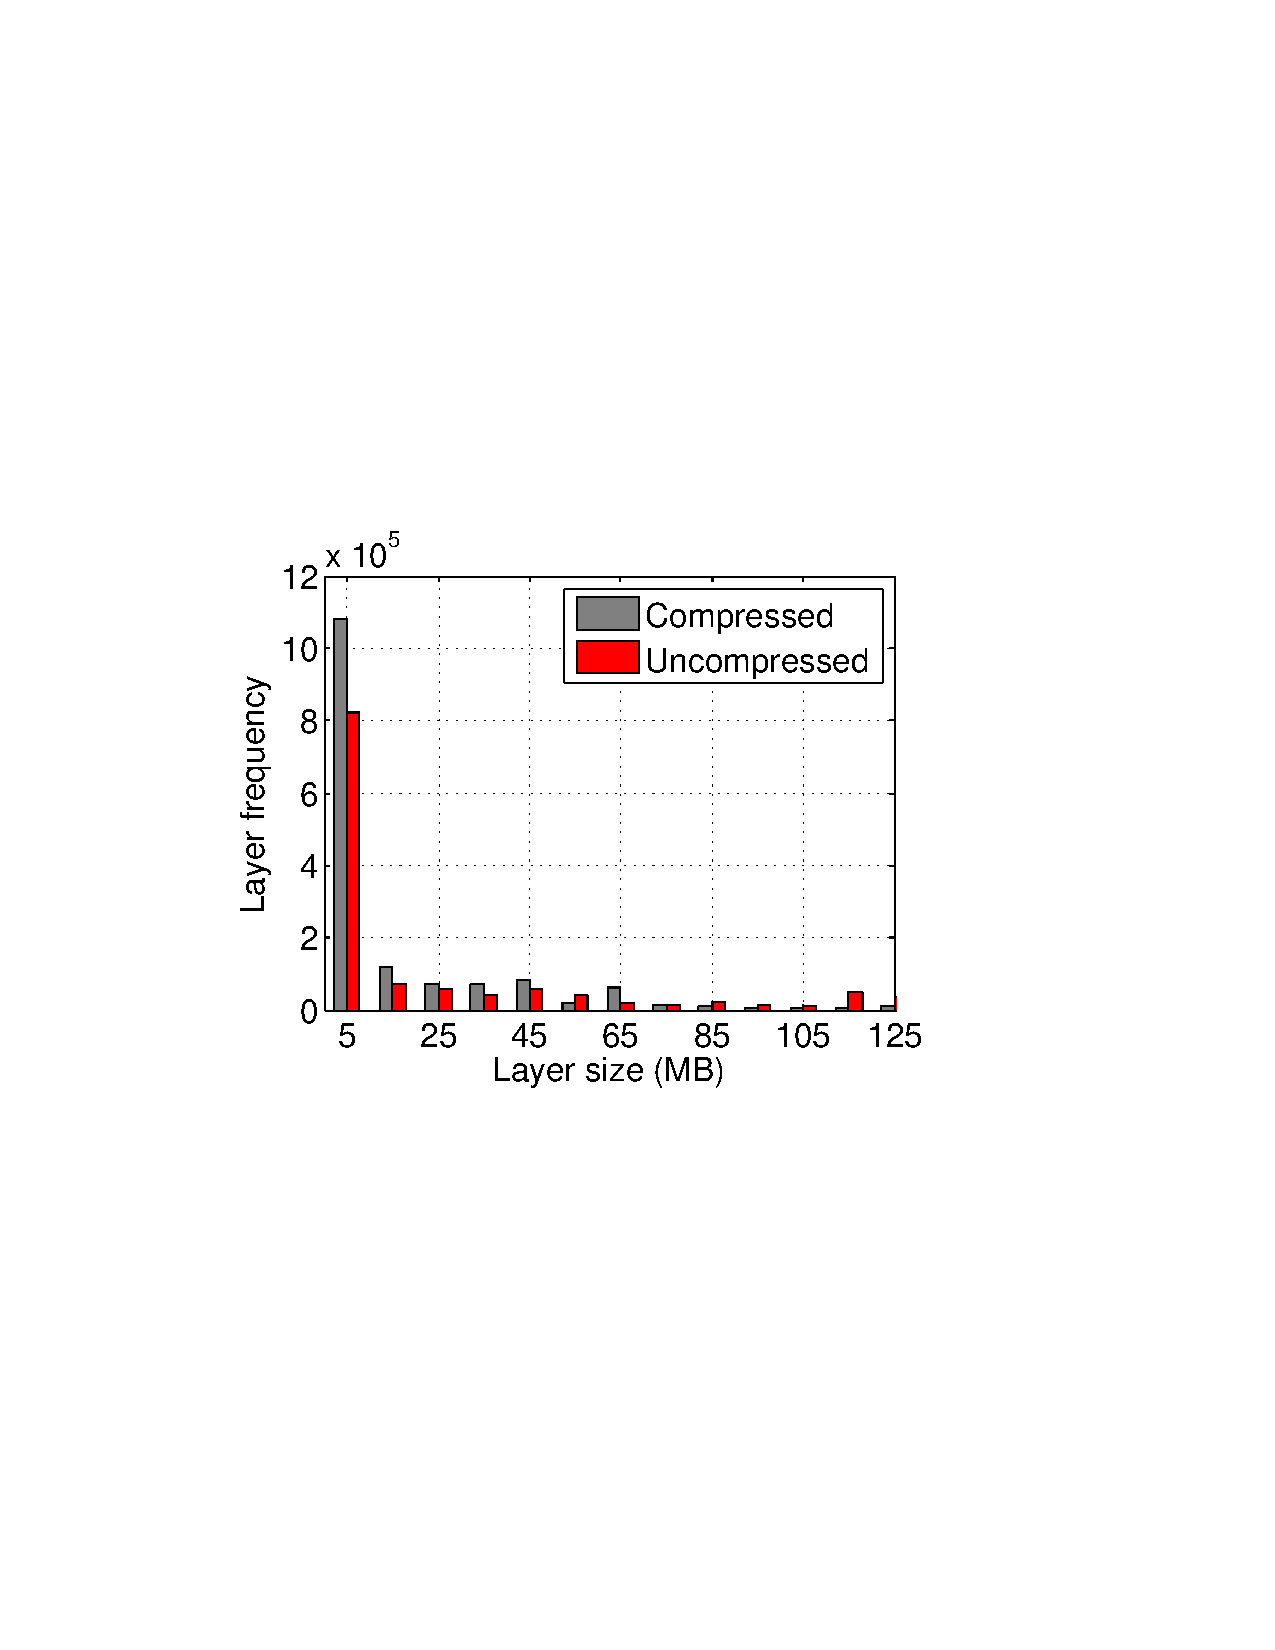
\includegraphics[width=0.213\textwidth]{graphs/hist_layer_size.pdf}
	}
	\caption{Layer size distribution
	\vcomment{Let's use CLS, ALS, and FLS abreviations\nancomment{addressed}}.
	\vcomment{CLS size should go first}.
	\vcomment{We need to use different types of lines (solid, dotted, etc.)
		or markers (round, triangular)}.
	\vcomment{In figure B it is not clear to which bar group corresponds
		  to which layer size. I suggest to try to rotate the graph
		  by 90 grads to fit all layer size labels.\nancomment{aligned label with bar}}
	}
	\label{fig-layer-size}
\end{figure}

%
%We found that most layers'compression ratio is really lower (?) while most of layers have a smaller size. 
%So how about we use archiving instead of compression if the network speed is higher (?GB/s)?

%\paragraph{Network transfer speed is high!}

%\subsubsection{File-level content addressable storage for cold layers}




%\begin{table} 
%	\centering 
%	\scriptsize  
%	%\begin{minipage}{.5\linewidth}
%	\caption{Summary of layer \& image characterization} \label{tbl:redundant_ratio} 
%	\begin{tabular}{|l|l|l|l|l|}%p{0.14\textwidth} 
%		\hline 
%		% after \\: \hline or \cline{col1-col2} \cline{col3-col4} ... 
%		% after \\: \hline or \cline{col1-col2} \cline{col3-col4} ... 
%		Metrics & max & min & median & avg.\\
%		\hline
%		Compressed layer size &   &   &   &  \\
%		\hline
%		Uncompressed layer size &   &   &    &  \\
%		\hline
%		Archival size &  &  & & \\
%		\hline
%		Compression ratio &   &   &    &  \\
%		\hline
%		Layer pull cnt. &  &  & & \\
%		\hline
%		File cnt. per layer &  &  & & \\
%		\hline
%		Dir. cnt. per layer &  &  & & \\
%		\hline
%		Layer depth &  &  & & \\
%		\hline
%		\hline
%		Compressed image size &  &  & & \\
%		\hline
%		Uncompressed image size & &  &  & \\
%		\hline
%		Archival image size & &  &  & \\
%		\hline
%		Compression ratio &   &   &    &  \\
%		\hline
%		Image pull cnt.  &  &  & & \\
%		\hline
%		Layer cnt. per image  &  &  & & \\
%		\hline
%		Shared layer cnt. per image  &  &  & & \\
%		\hline
%		File cnt. per layer &  &  & & \\
%		\hline
%		Dir. cnt. per layer &  &  & & \\
%		\hline	
%	\end{tabular} 
%\end{table} 

%\subsection{Constructing shared layers for redundant directories/files}
%
%\paragraph{Smaller number of layers are shared among different images}
%\begin{figure}[!t]
	\centering
	\subfigure[CDF of layer reference count]{\label{fig_repeate_layer}
		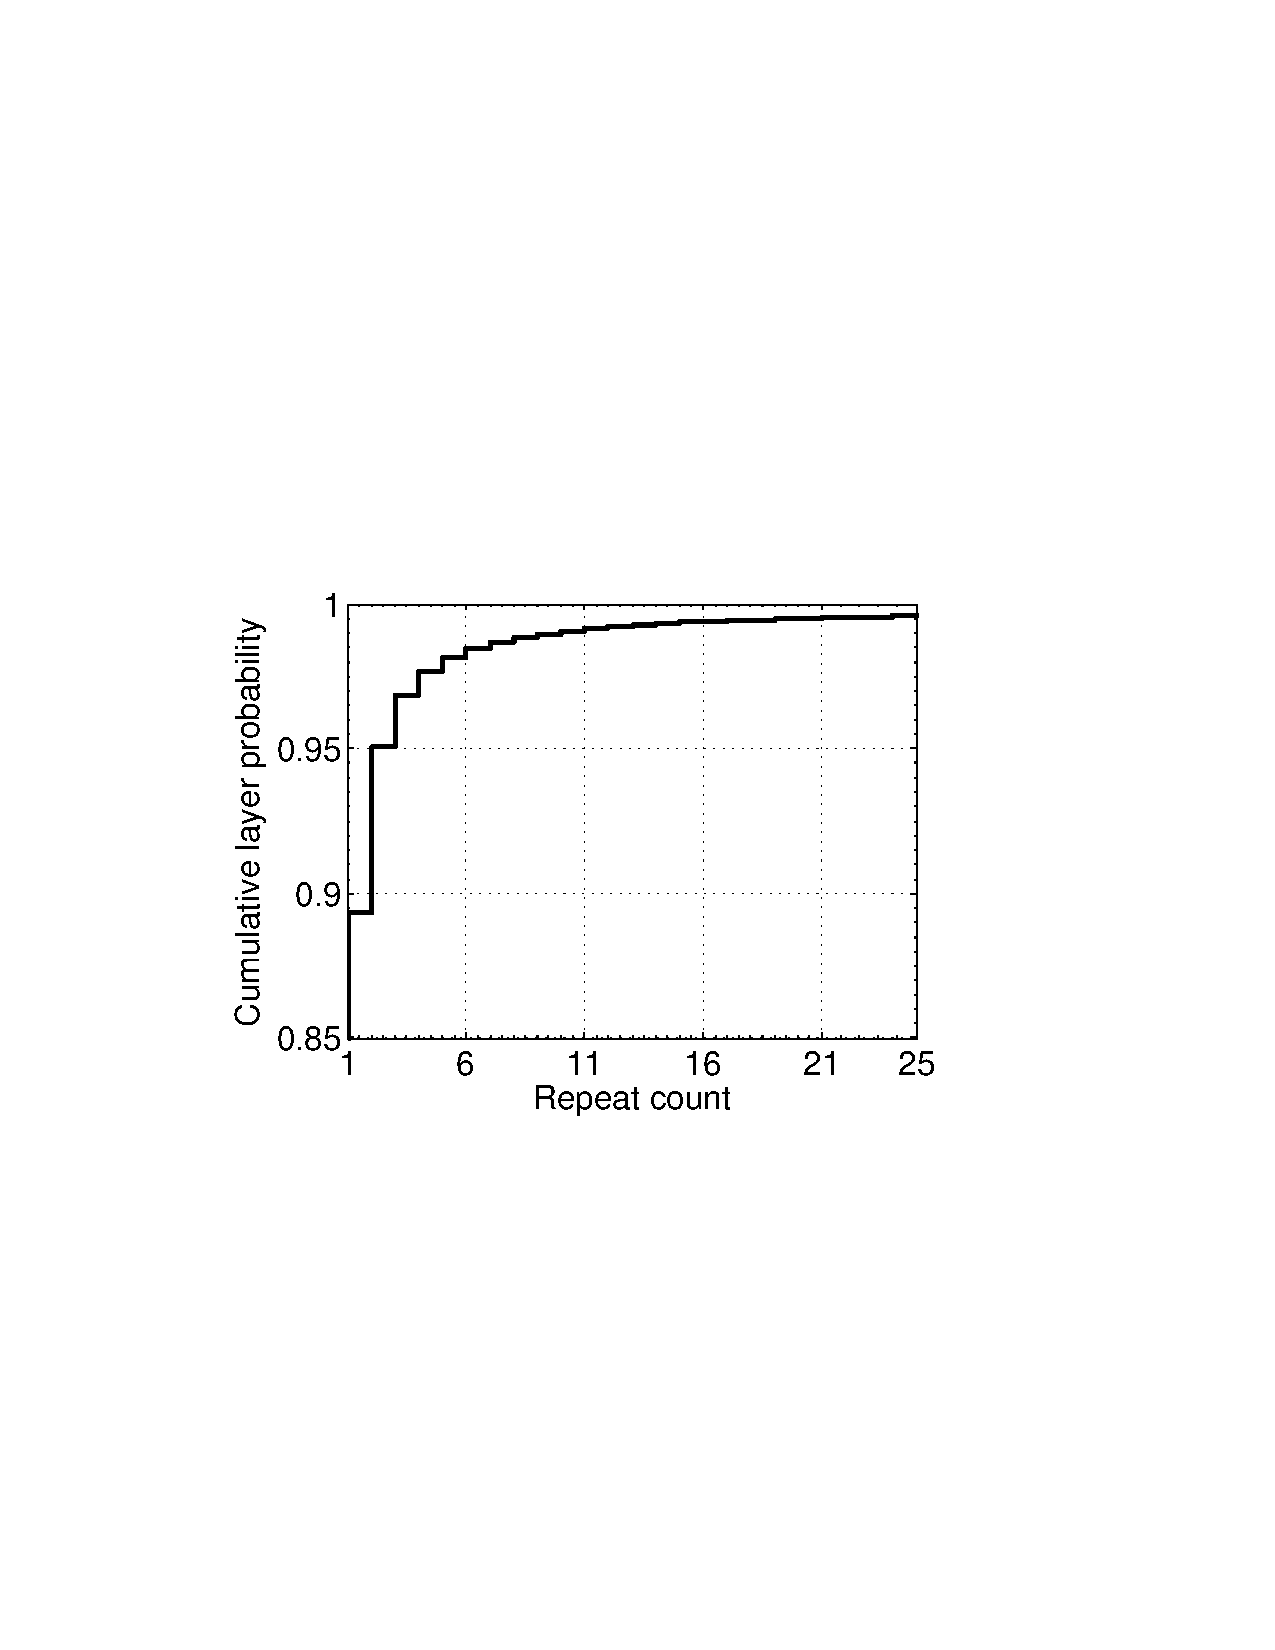
\includegraphics[width=0.23\textwidth]{graphs/repeate_layer.pdf}
	}
	\subfigure[Histogram of layer reference count]{\label{fig_hist_repeate_layer}
		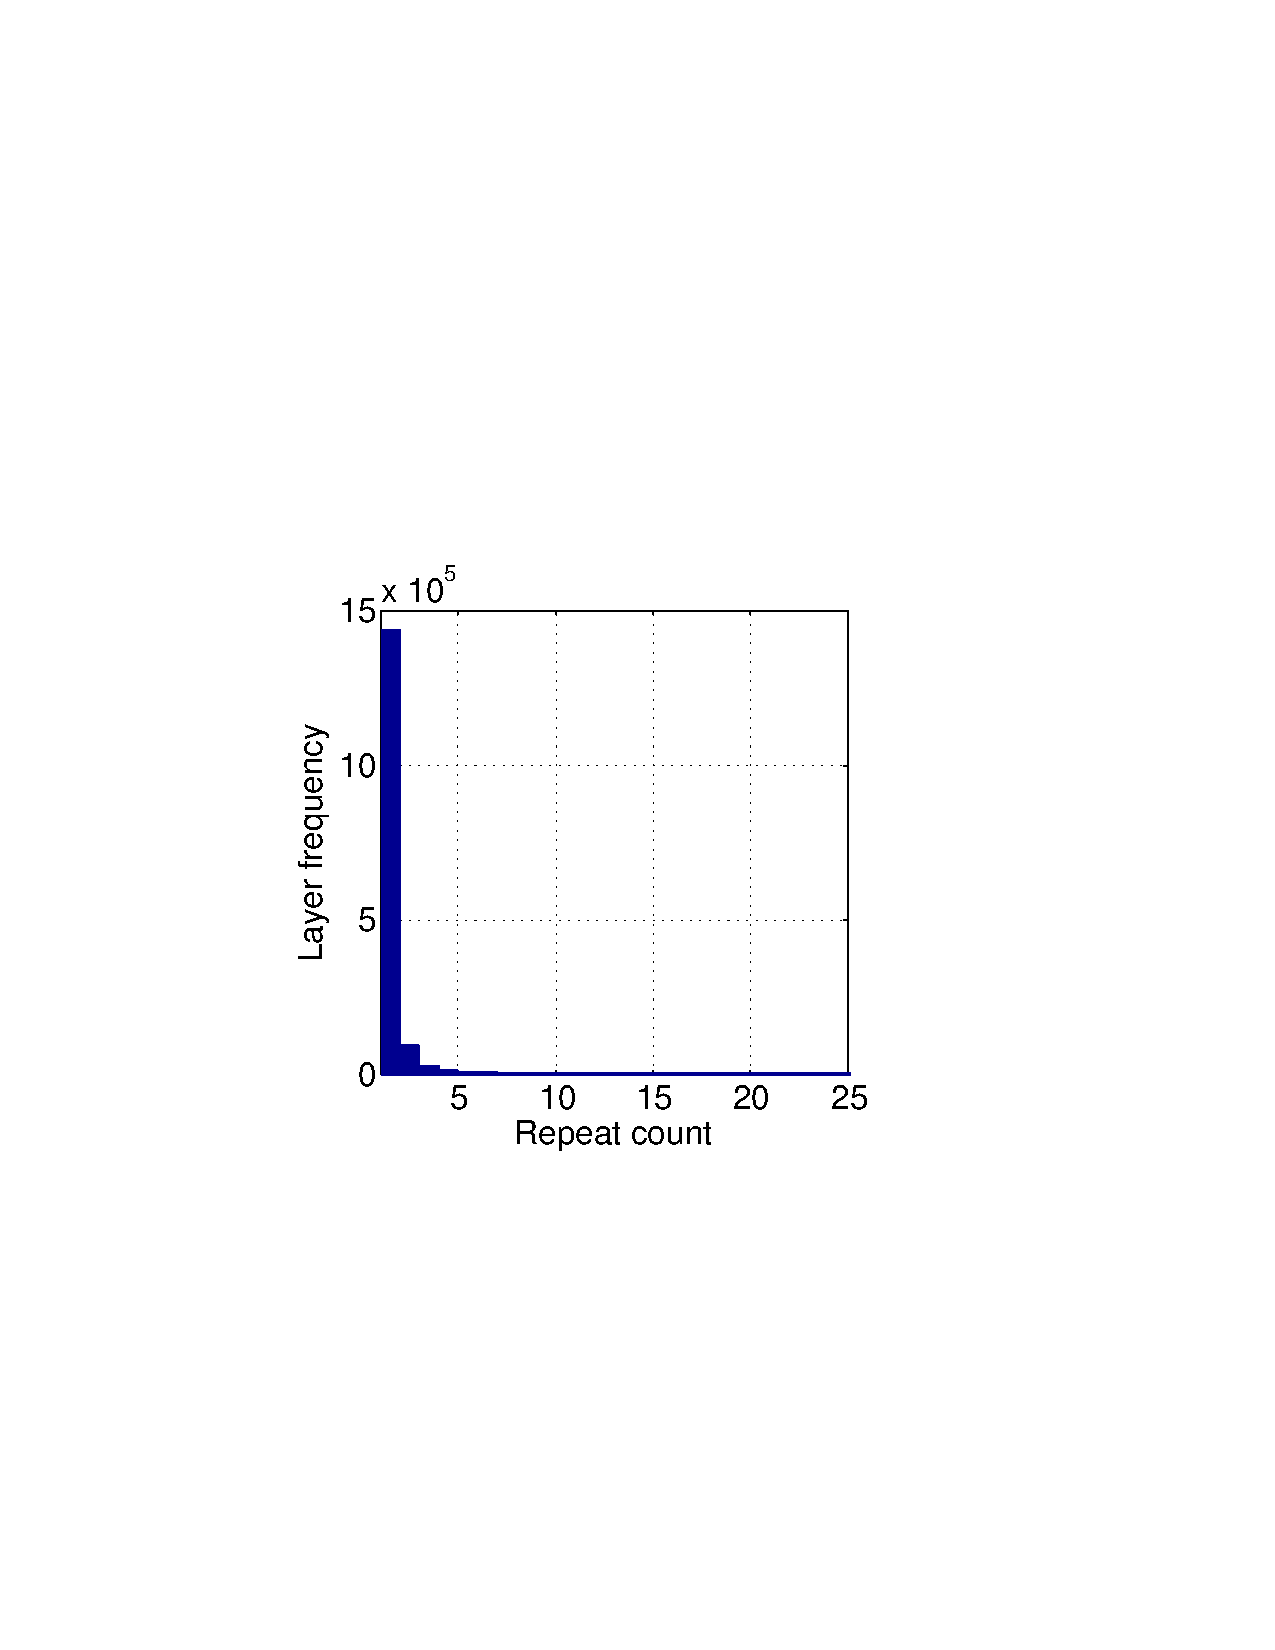
\includegraphics[width=0.223\textwidth]{graphs/hist_repeate_layer.pdf}
	}
	\caption{Layer reference counts across all images}
	\label{fig-repeat-layer-cnt}
\end{figure}
%
%\paragraph{Smaller pull latency than recompression model} the registry can prepare the reconstructed layers before users issue a pull request. But this model requires users to rebuild two layers.

%\subsubsection{Summary of Suggestions/trade-offs between dedup ratio and recompression overhead}
%
%\paragraph{1. using archiving instead of compression}
%\paragraph{2. using file-level dedup for cold images/layers}
%\paragraph{3. using file-level dedup economically}
%When to trigger file-level dedup?
%\paragraph{4. constructing shared layers for redundant dirs/files, for example,}
%%\subsection{Layer reconstruction model}
%%\subsubsection{Reconstruction overhead}
%%\subsubsection{Trade-offs between dedup ratio and reconstruction overhead}
%%\paragraph{Dedup ratio VS. Rebuild overhead}
%%\subsection{Evaluation results}